% !Mode:: "TeX:UTF-8"%確保文檔utf-8編碼
\documentclass[tikz,border=2pt]{standalone}
\usepackage{tikz-3dplot}
\begin{document}
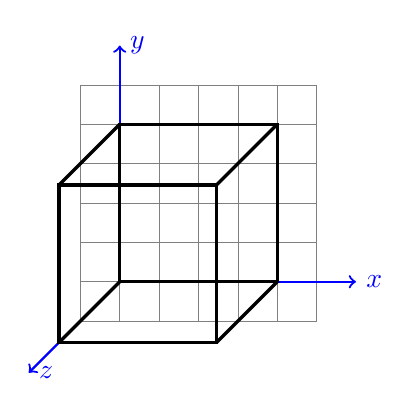
\begin{tikzpicture}
		[cube/.style={very thick,black},
			grid/.style={very thin,gray},
			axis/.style={->,blue,thick}]

	%draw a grid in the x-y plane
	\foreach \x in {-0.5,0,...,2.5}
		\foreach \y in {-0.5,0,...,2.5}
		{
			\draw[grid] (\x,-0.5) -- (\x,2.5);
			\draw[grid] (-0.5,\y) -- (2.5,\y);
		}
			
	%draw the axes
	\draw[axis] (0,0,0) -- (3,0,0) node[anchor=west]{$x$};
	\draw[axis] (0,0,0) -- (0,3,0) node[anchor=west]{$y$};
	\draw[axis] (0,0,0) -- (0,0,3) node[anchor=west]{$z$};

	%draw the top and bottom of the cube
	\draw[cube] (0,0,0) -- (0,2,0) -- (2,2,0) -- (2,0,0) -- cycle;
	\draw[cube] (0,0,2) -- (0,2,2) -- (2,2,2) -- (2,0,2) -- cycle;
	
	%draw the edges of the cube
	\draw[cube] (0,0,0) -- (0,0,2);
	\draw[cube] (0,2,0) -- (0,2,2);
	\draw[cube] (2,0,0) -- (2,0,2);
	\draw[cube] (2,2,0) -- (2,2,2);
	
\end{tikzpicture}


\tdplotsetmaincoords{60}{125}
\begin{tikzpicture}
		[tdplot_main_coords,
			cube/.style={very thick,black},
			grid/.style={very thin,gray},
			axis/.style={->,blue,thick}]

	%draw a grid in the x-y plane
	\foreach \x in {-0.5,0,...,2.5}
		\foreach \y in {-0.5,0,...,2.5}
		{
			\draw[grid] (\x,-0.5) -- (\x,2.5);
			\draw[grid] (-0.5,\y) -- (2.5,\y);
		}
			

	%draw the axes
	\draw[axis] (0,0,0) -- (3,0,0) node[anchor=west]{$x$};
	\draw[axis] (0,0,0) -- (0,3,0) node[anchor=west]{$y$};
	\draw[axis] (0,0,0) -- (0,0,3) node[anchor=west]{$z$};

	%draw the top and bottom of the cube
	\draw[cube] (0,0,0) -- (0,2,0) -- (2,2,0) -- (2,0,0) -- cycle;
	\draw[cube] (0,0,2) -- (0,2,2) -- (2,2,2) -- (2,0,2) -- cycle;
	
	%draw the edges of the cube
	\draw[cube] (0,0,0) -- (0,0,2);
	\draw[cube] (0,2,0) -- (0,2,2);
	\draw[cube] (2,0,0) -- (2,0,2);
	\draw[cube] (2,2,0) -- (2,2,2);
	
\end{tikzpicture}


\end{document}